\section{100 - The $3n + 1$ problem}

\textbf{Problema:} dados $i$ y $j$, encontrar la longitud m\'axima del ciclo, seg\'un la sucesi\'on de Collatz, para todos los
n\'umeros entre $i$ y $j$, donde $i, j$ est\'an en el rango $[1,1\,000\,000)$.

\begin{figure}[H]
\centering
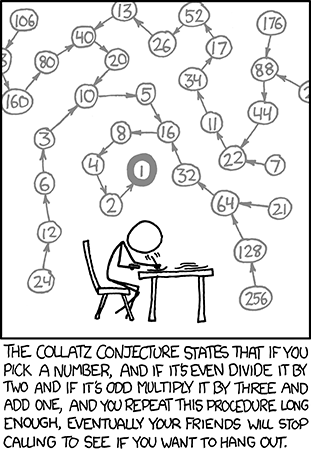
\includegraphics[scale=0.70]{./figuras/collatz_conjecture.png}
\end{figure}

\subsection{Resoluci\'on}
Para resolver este ejercicio se calculan los per\'iodos de todos los n\'umeros entre $i$ y $j$,
memorizando en un arreglo los per\'iodos ya calculados, para de esta manera no repetir c\'alculos.

Como estructura para memorizar, se utiliza un arreglo de un mill\'on de posiciones.
En general, para calcular el per\'iodo de los n\'umeros en $[1,n]$,
{\em podr\'ia} ser necesario calcular valores fuera de ese rango. La decisi\'on que tomamos fue no
memorizar el per\'iodo de los n\'umeros mayores que $999\,999$.
Ensayamos otras implementaciones que usaban un \texttt{map} para
memorizar los per\'iodos de todos los valores, pero en la pr\'actica
(adem\'as de cambiar la complejidad por usar un diccionario sobre \'arbol binario)
esto introduc\'ia un factor constante que lo hac\'ia bastante m\'as lento.

Si hubiera muchas b\'usquedas en intervalos grandes, se podr\'ia pensar en usar alguna
estructura de datos auxiliar que permitiera determinar r\'apidamente el
m\'aximo de un intervalo de un arreglo (como rmq). A modo de prueba, implementamos
una versi\'on simple de rmq (en la que una consulta cuesta $O(\sqrt{n})$), pero
el algorimo que usaba esa estructura tambi\'en resultaba comparativamente 
costoso en la pr\'actica.

%, porque usando un arreglo esto podr\'ia eventualmente necesitar una gran cantidad de memoria.
%%Es por esta raz�n que podr�a ocurrir que se repitan calculos, sin embargo creemos que el impacto que tienen esas repeticiones es despreciable.
%A la hora de realizar varias b\'usquedas, cada una se beneficia de los c\'a de periodos hechos en las anteriores. No obstante ello, si hay muchas busquedas grandes, todas recorren el rango entero. Esto podr�a hacerse de modo mas eficiente a fin de reducir el tiempo de las busquedas, sin embargo consideramos que eso escapa al problema.

Como observaci\'on adicional, se puede ver que, si $i \leq \lfloor j / 2 \rfloor$, no es
necesario buscar el m\'aximo en todo el intervalo $[i,j]$,
porque todos los valores menores que $j / 2$ tienen a su doble
dentro del intervalo. Por lo cual, dado que $periodo(2x) = periodo(x) + 1$,
el valor m\'aximo no se alcanza antes de $\lceil j / 2 \rceil$.

\begin{algorithm}[H]
\begin{algorithmic}
\caption{M\'aximo per\'iodo en un intervalo}
\PARAMS{$i,j$: bordes del intervalo donde buscar (se asume $i \leq j$)}
\ENSURE{ $maximo$: largo del per\'iodo m�ximo}
\STATE $periodo_1 := 1$
\STATE $desde := max(i,\lceil j/2 \rceil)$
\STATE $maximo := 0$
\FOR{cada $n$ entre $desde$ y $j$}
  \STATE $maximo := max(maximo, periodo_n)$
\ENDFOR
%\RETURN $maximo$
\end{algorithmic}
\end{algorithm}

\begin{algorithm}[H]
\begin{algorithmic}
\caption{Per\'iodo de un n\'umero de acuerdo con la relaci\'on de Collatz}
\PARAMS{$i$: n\'umero cuyo per\'iodo interesa conocer}
\IF{$periodo_i$ est\'a memorizado}
  \RETURN valor memorizado
\ELSE
  \STATE $p := periodo_{i'} + 1$ donde $i'$ es el siguiente de $i$ seg\'un la relaci\'on de Collatz
  \STATE memorizar $periodo_i = p$ si corresponde
  \RETURN $p$
\ENDIF
\end{algorithmic}
\end{algorithm}

Con respecto a la complejidad, si se tiene como entrada el intervalo $[i,j]$ (asumiendo
$i \leq j$), se calcula el per\'iodo de a lo sumo $j - i + 1$ n�meros. Ahora bien, $O(j-i) \subseteq O(j)$.
En muchos casos, calcular el per\'iodo requiere pocos pasos, porque alcanza con
buscar en el arreglo un per\'iodo ya calculado en otro paso; pero esto no ocurre siempre.
Sea $P$ el per\'iodo m�ximo en el intervalo sobre el que se realiza la consulta. Como cota superior
para el peor caso, calcular cada per\'iodo requiere $P$ pasos. Por esta raz\'on, la complejidad
del algoritmo es $O(P \cdot j)$.
Esta cota es bastante pesimista, ya que muy pocas veces se hacen
$P$ c\'alculos por n�mero.

%En particular, una vez que ya se calcularon todos
%los per\'iodos, las posteriores b\'usquedas requieren $O(max(i,j))$, ya que
%s\'olo se debe buscar el m\'aximo entre los valores de un arreglo.
En particular, si se realizan $n$ consultas, la complejidad, calculada
de la manera anterior, ser\'ia $O(P \cdot \sum_{k=1}^{n}{j_k})$,
donde $[i_k,j_k]$ es el intervalo de la $k$-\'esima consulta.
Pero, dado que acceder a un elemento ya memorizado es $O(1)$, el costo
del algoritmo es a lo sumo el de inicializar todo el arreglo una vez
m\'as el de buscar el m\'aximo para responder cada consulta, es
decir $O(P \cdot j_{\max} + \sum_{k=1}^{n}{j_k})$, donde $j_{\max} = \max_k{j_k}$.

En el intervalo $[1,999\,999]$ el valor de $P$ es $525$. Sin embargo, en
general, $P$ no es f\'acil de acotar. De hecho, si se pudiera acotar siempre,
se habr\'ia resuelto la conjetura de Collatz.

\subsection{Implementaci�n}

\noindent
\ttfamily
\shorthandoff{"}\\
\hlstd{}\hlline{\ 1\ }\hldir{\#include\ $<$stdio.h$>$}\\
\hlline{\ 2\ }\hlstd{}\hldir{\#include\ $<$iostream$>$}\\
\hlline{\ 3\ }\hlstd{}\hldir{\#include\ $<$vector$>$}\\
\hlline{\ 4\ }\hlstd{}\hlkwa{using\ namespace\ }\hlstd{std}\hlsym{;}\\
\hlline{\ 5\ }\hlstd{}\\
\hlline{\ 6\ }\hlkwc{typedef\ }\hlstd{}\hlkwb{unsigned\ int\ }\hlstd{uint}\hlsym{;}\\
\hlline{\ 7\ }\hlstd{}\hlkwc{typedef\ }\hlstd{}\hlkwb{unsigned\ short\ }\hlstd{ushort}\hlsym{;}\\
\hlline{\ 8\ }\hlstd{}\\
\hlline{\ 9\ }\hldir{\#define\ Max\textunderscore memo\ 1000001}\\
\hlline{10\ }\hlstd{vector}\hlsym{$<$}\hlstd{ushort}\hlsym{$>$\ }\hlstd{}\hlkwd{d}\hlstd{}\hlsym{(}\hlstd{Max\textunderscore memo}\hlsym{,\ }\hlstd{}\hlnum{0}\hlstd{}\hlsym{);}\\
\hlline{11\ }\hlstd{}\\
\hlline{12\ }\hldir{\#define\ memorizado(x)\ ((x)\ $<$\ Max\textunderscore memo\ \&\&\ d{[}(x){]}\ !=\ 0)}\\
\hlline{13\ }\hlstd{}\hldir{\#define\ next(n)\ ((n)\ \%\ 2\ ==\ 0\ ?\ (n)\ /\ 2\ :\ 3\ {*}\ (n)\ +\ 1)}\\
\hlline{14\ }\hlstd{\\
\hlline{15\ }ushort\ }\hlkwd{periodo}\hlstd{}\hlsym{(}\hlstd{uint\ n}\hlsym{)\ \{}\\
\hlline{16\ }\hlstd{\ }\hlkwa{if\ }\hlstd{}\hlsym{(}\hlstd{}\hlkwd{memorizado}\hlstd{}\hlsym{(}\hlstd{n}\hlsym{))\ \{}\\
\hlline{17\ }\hlstd{}\hlstd{\ \ }\hlstd{}\hlkwa{return\ }\hlstd{d}\hlsym{{[}}\hlstd{n}\hlsym{{]};}\\
\hlline{18\ }\hlstd{\ }\hlsym{\}\ }\hlstd{}\hlkwa{else\ }\hlstd{}\hlsym{\{}\\
\hlline{19\ }\hlstd{}\hlstd{\ \ }\hlstd{ushort\ p\ }\hlsym{=\ }\hlstd{}\hlkwd{periodo}\hlstd{}\hlsym{(}\hlstd{}\hlkwd{next}\hlstd{}\hlsym{(}\hlstd{n}\hlsym{))\ +\ }\hlstd{}\hlnum{1}\hlstd{}\hlsym{;}\\
\hlline{20\ }\hlstd{}\hlstd{\ \ }\hlstd{}\hlkwa{if\ }\hlstd{}\hlsym{(}\hlstd{n\ }\hlsym{$<$\ }\hlstd{Max\textunderscore memo}\hlsym{)\ \{}\\
\hlline{21\ }\hlstd{}\hlstd{\ \ \ }\hlstd{d}\hlsym{{[}}\hlstd{n}\hlsym{{]}\ =\ }\hlstd{p}\hlsym{;}\\
\hlline{22\ }\hlstd{}\hlstd{\ \ }\hlstd{}\hlsym{\}}\\
\hlline{23\ }\hlstd{}\hlstd{\ \ }\hlstd{}\hlkwa{return\ }\hlstd{p}\hlsym{;}\\
\hlline{24\ }\hlstd{\ }\hlsym{\}}\\
\hlline{25\ }\hlstd{}\hlsym{\}}\\
\hlline{26\ }\hlstd{\\
\hlline{27\ }ushort\ }\hlkwd{resolver}\hlstd{}\hlsym{(}\hlstd{uint\ x}\hlsym{,\ }\hlstd{uint\ y}\hlsym{)\{}\\
\hlline{28\ }\hlstd{\ ushort\ res\ }\hlsym{=\ }\hlstd{}\hlnum{0}\hlstd{}\hlsym{;}\\
\hlline{29\ }\hlstd{\ uint\ i\ }\hlsym{=\ }\hlstd{}\hlkwd{min}\hlstd{}\hlsym{(}\hlstd{x}\hlsym{,}\hlstd{y}\hlsym{);}\\
\hlline{30\ }\hlstd{\ uint\ sup\ }\hlsym{=\ }\hlstd{}\hlkwd{max}\hlstd{}\hlsym{(}\hlstd{x}\hlsym{,}\hlstd{y}\hlsym{);}\\
\hlline{31\ }\hlstd{\ ushort\ aux}\hlsym{;}\\
\hlline{32\ }\hlstd{\ i\ }\hlsym{=\ }\hlstd{}\hlkwd{max}\hlstd{}\hlsym{(}\hlstd{sup}\hlsym{/}\hlstd{}\hlnum{2}\hlstd{}\hlsym{,}\hlstd{i}\hlsym{);}\\
\hlline{33\ }\hlstd{\\
\hlline{34\ }\ }\hlkwa{while}\hlstd{}\hlsym{(}\hlstd{i\ }\hlsym{$<$=\ }\hlstd{sup}\hlsym{)\{}\\
\hlline{35\ }\hlstd{}\hlstd{\ \ }\hlstd{aux\ }\hlsym{=\ }\hlstd{}\hlkwd{periodo}\hlstd{}\hlsym{(}\hlstd{i}\hlsym{);}\\
\hlline{36\ }\hlstd{}\hlstd{\ \ }\hlstd{}\hlkwa{if\ }\hlstd{}\hlsym{(}\hlstd{aux\ }\hlsym{$>$\ }\hlstd{res}\hlsym{)\{}\\
\hlline{37\ }\hlstd{}\hlstd{\ \ \ }\hlstd{res\ }\hlsym{=\ }\hlstd{aux}\hlsym{;}\\
\hlline{38\ }\hlstd{}\hlstd{\ \ }\hlstd{}\hlsym{\}}\\
\hlline{39\ }\hlstd{}\hlstd{\ \ }\hlstd{i}\hlsym{++;}\\
\hlline{40\ }\hlstd{\ }\hlsym{\}}\\
\hlline{41\ }\hlstd{\ }\hlkwa{return\ }\hlstd{res}\hlsym{;}\\
\hlline{42\ }\hlstd{}\hlsym{\}}\\
\hlline{43\ }\hlstd{}\\
\hlline{44\ }\hlkwb{int\ }\hlstd{}\hlkwd{main}\hlstd{}\hlsym{(}\hlstd{}\hlkwb{int\ }\hlstd{argc}\hlsym{,\ }\hlstd{}\hlkwb{char\ }\hlstd{}\hlsym{{*}{*}}\hlstd{argv}\hlsym{)}\\
\hlline{45\ }\hlstd{}\hlsym{\{}\\
\hlline{46\ }\hlstd{\ uint\ x}\hlsym{,\ }\hlstd{y}\hlsym{;}\\
\hlline{47\ }\hlstd{\ d}\hlsym{{[}}\hlstd{}\hlnum{1}\hlstd{}\hlsym{{]}\ =\ }\hlstd{}\hlnum{1}\hlstd{}\hlsym{;}\\
\hlline{48\ }\hlstd{\ }\hlkwa{while\ }\hlstd{}\hlsym{(}\hlstd{}\hlkwd{scanf}\hlstd{}\hlsym{(}\hlstd{}\hlstr{"\%u\ \%u"}\hlstd{}\hlsym{,\&}\hlstd{x}\hlsym{,\&}\hlstd{y}\hlsym{)==}\hlstd{}\hlnum{2}\hlstd{}\hlsym{)\ \{}\\
\hlline{49\ }\hlstd{}\hlstd{\ \ }\hlstd{cout\ }\hlsym{$<$$<$\ }\hlstd{x\ }\hlsym{$<$$<$}\hlstd{}\hlstr{"\ "}\hlstd{}\hlsym{$<$$<$\ }\hlstd{y\ }\hlsym{$<$$<$}\hlstd{}\hlstr{"\ "}\hlstd{\ }\hlsym{$<$$<$\ }\hlstd{}\hlkwd{resolver}\hlstd{}\hlsym{(}\hlstd{x}\hlsym{,\ }\hlstd{y}\hlsym{)\ $<$$<$\ }\hlstd{endl}\hlsym{;}\\
\hlline{50\ }\hlstd{\ }\hlsym{\}}\\
\hlline{51\ }\hlstd{\ }\hlkwa{return\ }\hlstd{}\hlnum{0}\hlstd{}\hlsym{;}\\
\hlline{52\ }\hlstd{}\hlsym{\}}\\
\hlline{53\ }\hlstd{}\\
\mbox{}
\normalfont
\shorthandon{"}


